\newpage
\section{Auswertung}
\label{sec:Auswertung}

\subsection{Vorbereitung}
\subsubsection{Vorbereitungsaufgaben}

  Als Vorbereitung auf die Versuchsreihe, werden Literaturwerte zur Dichte und Schallgeschwindigkeit verschiedener
  Materialien recherchiert. Anschließend wird die Impedanz mithilfe von $Z = \rho \cdot c$ ausgerechnet.\\
  Die Werte lassen sich in \autoref{tab:Literaturwerte} finden.
  \begin{table}
    \centering
    \caption{Literaturwerte und akustische Impedanzen verschiedener Materialien.}
    \label{tab:Literaturwerte}
    \begin{tabular}{c | l l l}
      Material & Schallgeschwindigkeit $c$ / $\frac{\mathrm{m}}{\mathrm{s}}$ & Dichte $\rho$ / $\frac{\mathrm{g}}{\mathrm{cm}^3}$ & Akustische Impendanz $Z$ / $\frac{\mathrm{kg}}{\mathrm{sm}^2} \cdot 10^6$\\
        \midrule
          Luft    & 331 \cite{medizinphysik}     & 1,300 $\cdot 10^{-3}$ \cite{medizinphysik}& 4,3 $\cdot 10^{-4}$ \\
          Wasser  & 1492 \cite{medizinphysik}    & 0,9982 \cite{medizinphysik}               & 1,48 \\
          Blut    & 1530 \cite{medizinphysik}    & 1,03   \cite{medizinphysik}               & 1,56  \\
          Knochen & 3600 \cite{medizinphysik}    & 1,7    \cite{medizinphysik}               & 6,12  \\
          Acryl   & 2730 \cite{thiemann}        & 1,189  \cite{imeter}                       & 3,25  \\
        \bottomrule
      \end{tabular}
  \end{table}
  Anschließend wird die Wellenlänge und die Periode einer 2 MHz Schwingung in Acryl ausgerechnet.
  \begin{align*}
    \lambda = \frac{c}{f} = 1,365 \cdot 10^{-3} \, \mathrm{m} \\
    T = \frac{1}{f} = 0,5 \cdot 10^{-6} \, \mathrm{s}
  \end{align*}

\subsubsection{Kennenlernen und Einstellen des Programms}

  Mit der Schieblehre wird die Dicke einer gegebenen Acrylplatte gemessen. Diese beträgt $d=(9,95 \pm 0,05) \, \cdot 10^{-3} \, \mathrm{m}$.\\
  Anschließend wird ein A-Scan durchgeführt, welcher die Graphik in \autoref{fig:1cmAcrylplatt} erzeugt.\\
  \begin{figure}
    \centering
    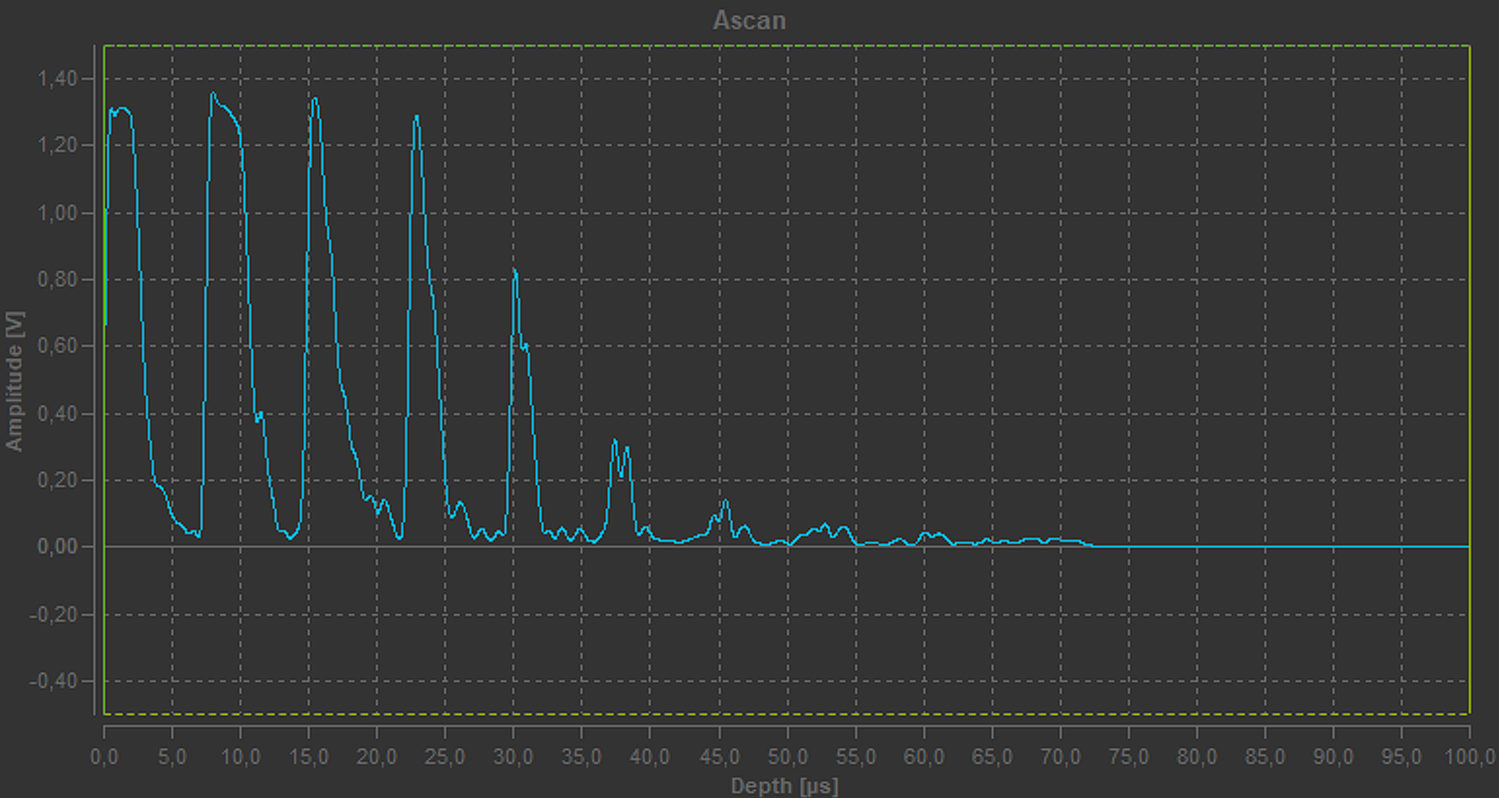
\includegraphics[width=15cm]{messwerte/Vorbereitung/AScan_Vorbereitung.png}
    \caption{A-Scan der 1 cm dicken Acrylplatte.}
    \label{fig:1cmAcrylplatt}
  \end{figure}
  In der Abbildung lassen sich fünf Schwingungen besonders gut erkennen. Von diesen Schwingungen wird die Laufzeit und
  Amplitude mittels importierter Daten aus dem Programm bestimmt und in \autoref{tab:LaufzeitenUndAmplituden} aufgelistet.
  \begin{table}
    \centering
    \caption{Laufzeiten und Amplituden der ersten fünf Schwingungen.}
    \label{tab:LaufzeitenUndAmplituden}
    \begin{tabular}{c | c c}
      Schwingung & Laufzeit $t$ / $\si{\micro\second}$ & Amplitude $A$ / $\si{\volt}$ \\
        \midrule
          1 & 7,12  & 1,316 \\
          2 & 14,40  & 1,366 \\
          3 & 21,80  & 1,340 \\
          4 & 29,44  & 1,297 \\
          5 & 36,66  & 0,880 \\
        \bottomrule
      \end{tabular}
  \end{table}
  Aus den gemessenen Daten wird der Mittelwert der Laufzeiten der einzelnen Impulsreflexionen (Zeitdifferenz zum vorherigen Impuls)
  und anschließend die Schallgeschwindigkeit mittels \autoref{eqn:Strecke} bestimmt.\\
  Mittelwert der Laufzeit:
  \begin{align*}
    t &= (7,33 \pm 0,09) \, \si{\micro\second} \\
    c &= \frac{2s}{t} \\
      &= (2714,87 \pm 13,64) \, \si{\meter\per\second}
  \end{align*}
  Die Unsicherheit wurde mittels Gaußscher Fehlerfortpflanzung bestimmt. Die Schallgeschwindigkeit in Acryl lautet somit
  $c_{\mathrm{Acryl}} = (2714,87 \pm 13,64) \, \si{\meter\per\second}$.\\
  Nun wird zwischen den Anzeigemodi $AM$, $HF$ und $AM + HF$ gewechselt und Bilder der Modi aufgezeichnet. Die Bilder sind 
  in \autoref{Modi} gezeigt.
  \begin{figure}
    \centering
    \begin{subfigure}[b]{0.3\textwidth}
      \centering
      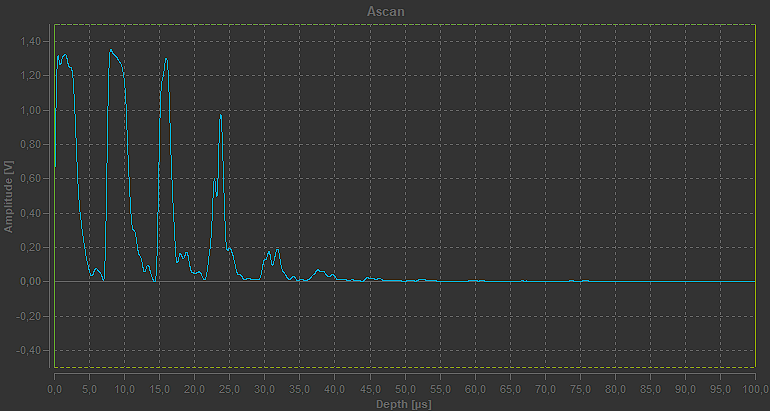
\includegraphics[width=4.5cm]{messwerte/Vorbereitung/Amp.png}
      \caption{$AM$ Modus}
    \end{subfigure}
    ~
    \begin{subfigure}[b]{0.3\textwidth}
      \centering
      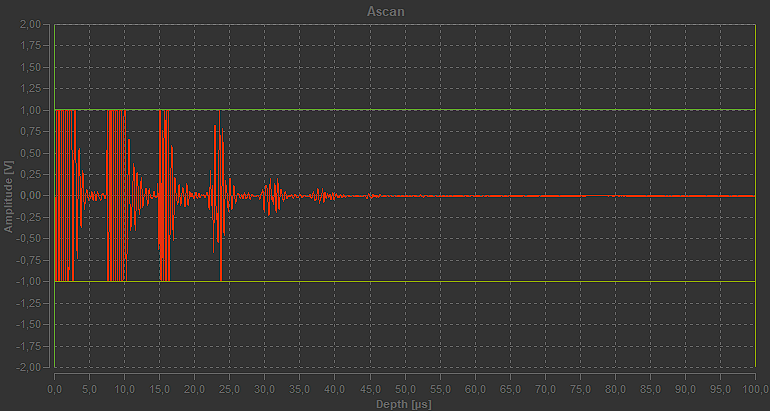
\includegraphics[width=4.5cm]{messwerte/Vorbereitung/HF.png}
      \caption{$HF$ Modus}
    \end{subfigure}
    ~
    \begin{subfigure}[b]{0.3\textwidth}
      \centering
      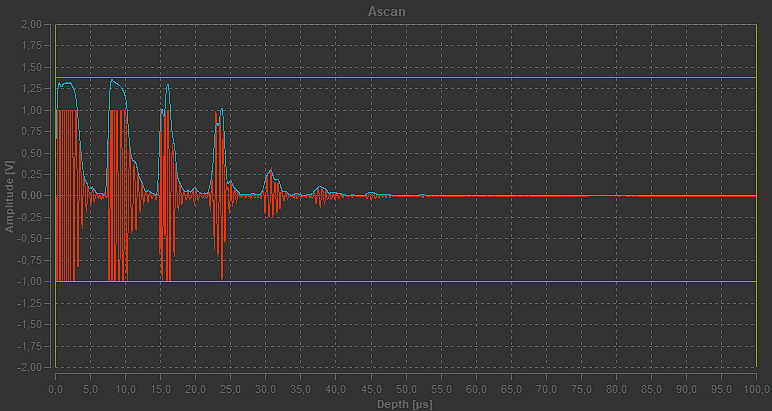
\includegraphics[width=4.5cm]{messwerte/Vorbereitung/HF+Amp.png}
      \caption{$AM + HF$ Modus}
    \end{subfigure}
    \caption{Alle drei verschiedenen Anzeigemodi}
    \label{Modi}
  \end{figure}

  Es lässt sich erkennen, dass im $HF$-Modus jede einzelne Schwingung angezeigt wird, während
  im $AM$-Modus jeweils nur die positiven Amplituden jener Schwingungen angezeigt werden. Im $AM + HF$-Modus
  werden jene zwei Modi kombiniert ausgegeben.\\
  Je nach Versuchsteil wird ein anderer Modus verwendet.\\
  Als nächstes wird der $AM + HF$-Modus eingeschaltet und bei einer $2 \, \si{\mega\hertz}$ Schwingung die Periode einer Schwingung
  ausgerechnet. Dafür wird über fünf Perioden hinweg gemittelt. Der verwendete Bereich ist mittels grünen Balken 
  in \autoref{fig:T} eingezeichnet.
  \begin{figure}
    \centering
    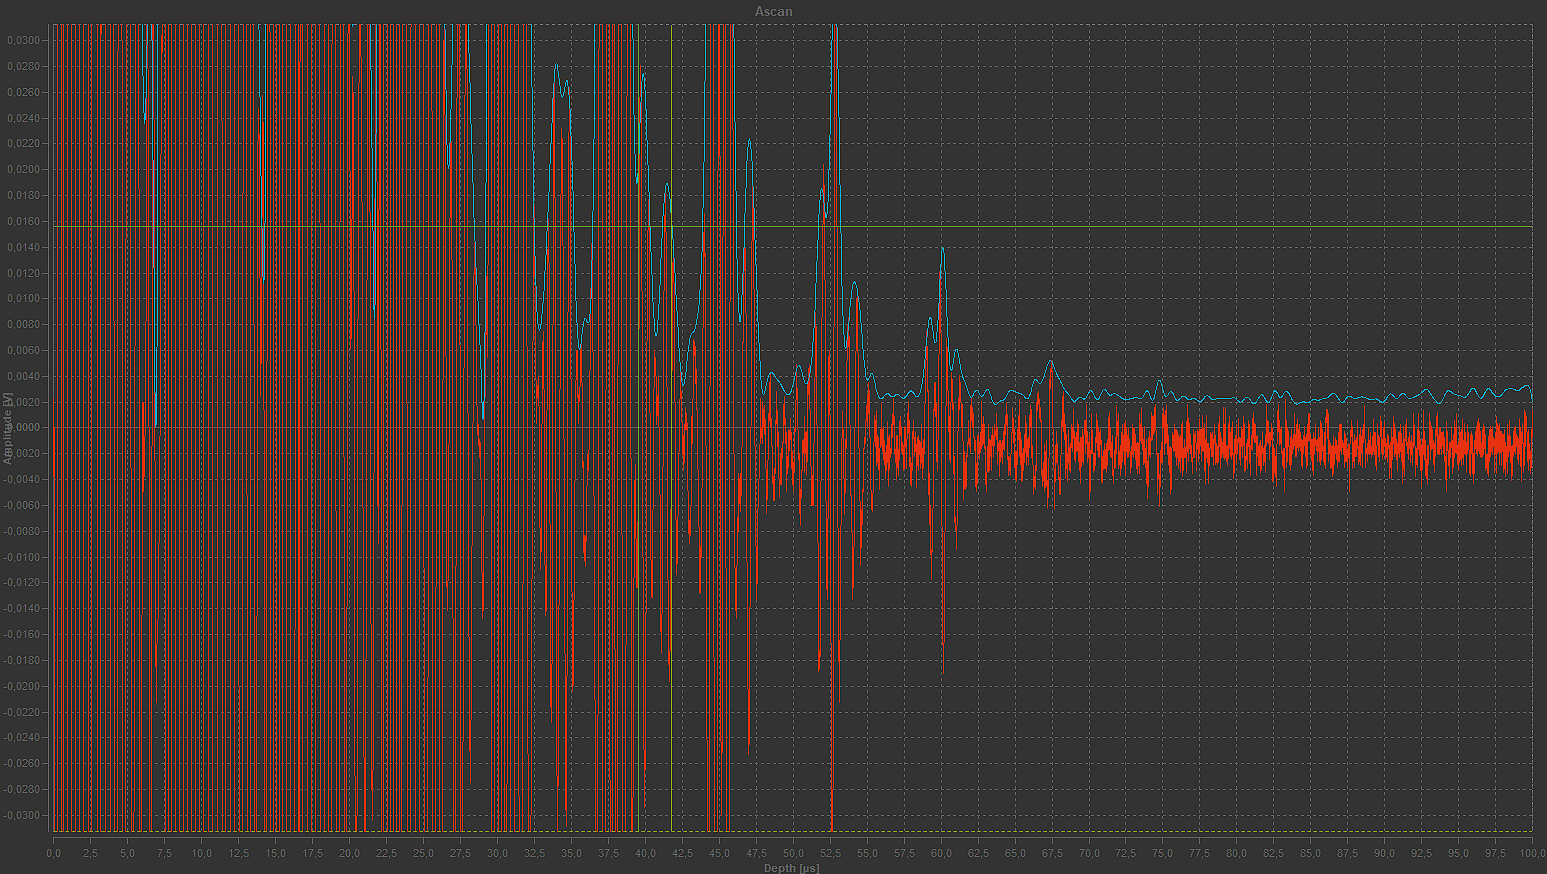
\includegraphics[width=15cm]{messwerte/Vorbereitung/T.png}
    \caption{2 MHz Schwingung im $AM + HF$-Modus angezeigt.}
    \label{fig:T}
  \end{figure}
  Die fünf Perioden zusammenaddiert haben eine Länge von $T_5 =2,2 \, \si{\micro\second}$. Dieser Messwert wird
  durch fünf geteilt, um die Länge einer Periode zu erhalten: $T_1 = \frac{2,2}{5} \, \si{\micro\second} = 0,44 \, \si{\micro\second}$.
  Daraus lässt sich nun die Wellenlänge und Frequenz der Schwinung in Acryl berechnen:
  \begin{align*}
    f &= \frac{1}{T} = 2 272 727,27 \, \si{\per\second} = 2,3 \, \mathrm{MHz}\\
    \lambda &= (1,19 \pm 0,01) \cdot 10^{-3} \, \si{\meter}
  \end{align*}
  Mittels der Tiefenmessung des Programms wird für die Acrylplatte eine Dicke von 1 cm gemessen.

\subsection{Ausmessen der verwendeten Acrylzylinder}

  Insgesamt stehen vier verschiedene Größen von Acrylzylindern zur Verfügung. Diese werden alle mit einer Schieblehre
  ausgemessen. Die Messwerte sind in \autoref{tab:Zylinder} eingetragen. Die Schieblehre hat eine Messungenauigkeit von
  0,05 mm.

  \begin{table}
    \centering
    \caption{Messwerte der vier verschiedenen Acrylzylinder.}
    \label{tab:Zylinder}
    \begin{tabular}{c | c c}
      Zylindernummer & Höhe $h$ / $\si{\milli\meter}$ & Durchmesser $d$ / $\si{\milli\meter}$ \\
        \midrule
          1 & 120,90 & 40,00 \\
          2 & 80,50  & 40,10 \\
          3 & 61,55  & 40,45 \\
          4 & 40,45  & 40,15 \\
        \bottomrule
      \end{tabular}
  \end{table}

\subsection{Schallgeschwindigkeitsbestimmung mit dem Impuls-Echo-Verfahren}

  In dieser Versuchsreihe werden die vier Zylinder mittels Impuls-Echo-Verfahren beschallt. Zudem wird noch
  ein 10 cm großer Zylinder aus den einzelnen Zylindern gebaut und beschallt. Die Messwerte lassen sich in 
  \autoref{tab:EchoImpuls} finden.

  \begin{table}
    \centering
    \caption{Zur Bestimmung der Schallgeschwindigkeit mit Impuls-Echo-Verfahren aufgenommene Messwerte.}
    \label{tab:EchoImpuls}
    \begin{tabular}{c | c c c c}
      Höhe $l$ / $\si{\milli\meter}$ & Ausges. Imp. $U_{\mathrm{A}}$ / $\si{\volt}$ &  Startzeit $t_0$ / $\si{\micro\second}$ & Refklekt. Imp. $U_{\mathrm{R}}$ / $\si{\volt}$ & Endzeit $t_{\mathrm{R}}$ / $\si{\micro\second}$ \\
        \midrule
          40,45 & 1,318 & 1,260 & 1,250 & 30,26 \\
          61,55 & 1,318 & 1,280 & 0,619 & 46,04 \\
          80,50 & 1,319 & 1,240 & 0,304 & 59,50 \\
          102,00 & 1,318 & 1,260 & 0,068 & 75,34 \\
          120,90 & 1,319 & 1,260 & 1,193 & 88,56 \\
        \bottomrule
      \end{tabular}
  \end{table}

  $U_{\mathrm{A}}$ ist die Amplitude des ausgesendeten Impulses, $t_0$ der Zeitpunkt, wo die Amplitude des ausgesendeten Impulses
  gemessen wird, $U_{\mathrm{R}}$ die Amplitude des reflektierten Impulses und $t_{\mathrm{R}}$ der Zeitpunkt, wo die Amplitude des reflektierten
  Impulses gemessen wird.\\
  Mittels dieser Messwerte wird eine lineare Ausgleichsrechnung mit Python durchgeführt. Die Theoriekurve ergibt sich aus
  \autoref{eqn:Strecke} und einer Anpassungsschicht $d$ für die Sonde. Die Geradengleichung lautet also
  \begin{equation*}
    2l = c \cdot t + d.
  \end{equation*}
  $l$ ist die jeweilige Länge des Zylinders und $t = t_{\mathrm{R}} - t_0$ die Laufzeit der Schwingung.\\
  \begin{figure}
    \centering
    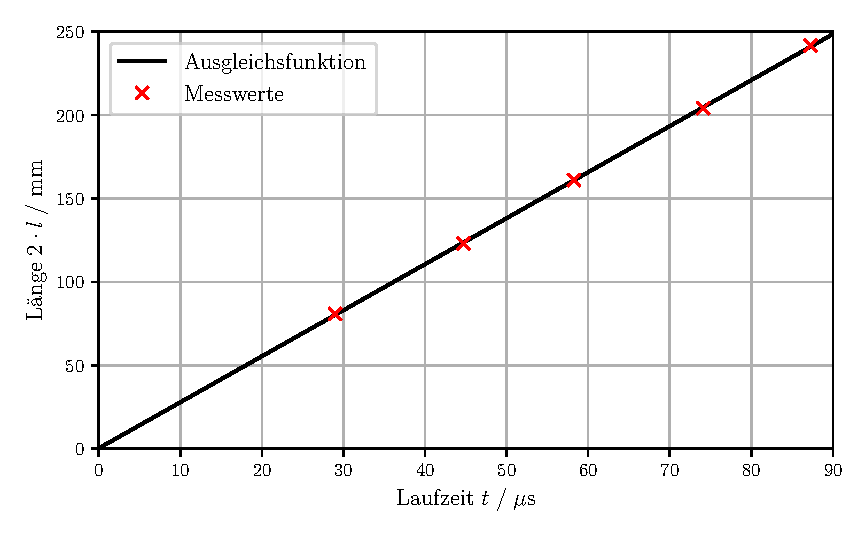
\includegraphics[width=15cm]{messwerte/ImpulsEcho.pdf}
    \caption{doppelte Zylinderhöhe $l$ geplottet gegen die Laufzeit $t$ beim Impuls-Echo-Verfahren.}
    \label{fig:ImpulsEcho}
  \end{figure}
  Mittels Python ergibt sich dann die Steigung und der y-Achsenabschnitt der Geraden. Die Steigung entspricht
  der Schallgeschwindigkeit in Acryl $c_{\mathrm{Acryl}}$ und der y-Achsenabschnitt entspricht der Anpassungsschicht $d$.\\
  \begin{align*}
    c_{\mathrm{Acryl}} &= (2,75895 \pm 0,01631) \, \si{\milli\meter\per\micro\second} &= (2758,95 \pm 16,31) \, \si{\meter\per\second} \\
    d &= (0,26 \pm 1,02) \, \si{\milli\meter} &= (0,26 \pm 1,02) \cdot 10^{-3} \, \si{\meter}
  \end{align*}
  Die Messwerte und Ausgleichsfunktion sind in \autoref{fig:ImpulsEcho} dargestellt.

\subsection{Schallgeschwindigkeitsbestimmung mit Durchschallungs-Verfahren}

  Für diese Versuchsreihe werden alle 4 Zylindergrößen horizontal platziert und mittels zwei Sonden durchschallt.\\
  Mit diesem Verfahren ergibt sich für die Strecke die Gleichung 
  \begin{equation*}
    l = c \cdot t + d,
  \end{equation*}
  da der Weg bis zur Singnalempfangung nur einmal zurückgelegt wird.\\
  Mittels A-Scan wird die Laufzeit des Impulses gemessen und in \autoref{tab:Durchschallung} aufgelistet.
  \begin{table}
    \centering
    \caption{Zur Bestimmung der Schallgeschwindigkeit mit Impuls-Echo-Verfahren aufgenommene Messwerte.}
    \label{tab:Durchschallung}
    \begin{tabular}{c | c c}
      Höhe $l$ / $\si{\milli\meter}$ & Startzeit $t_0$ / $\si{\micro\second}$ & Endzeit $t_{\mathrm{R}}$ / $\si{\micro\second}$ \\
        \midrule
        40   & 0,2 & 15,48\\
        60   & 0,2 & 23,78\\
        80   & 0,2 & 30,22\\
        120  & 0,2 & 44,76\\
        \bottomrule
      \end{tabular}
  \end{table}

  Es wird mit der obigen Gleichung eine Ausgleichsrechnung in Python durchgeführt.
  \begin{figure}
    \centering
    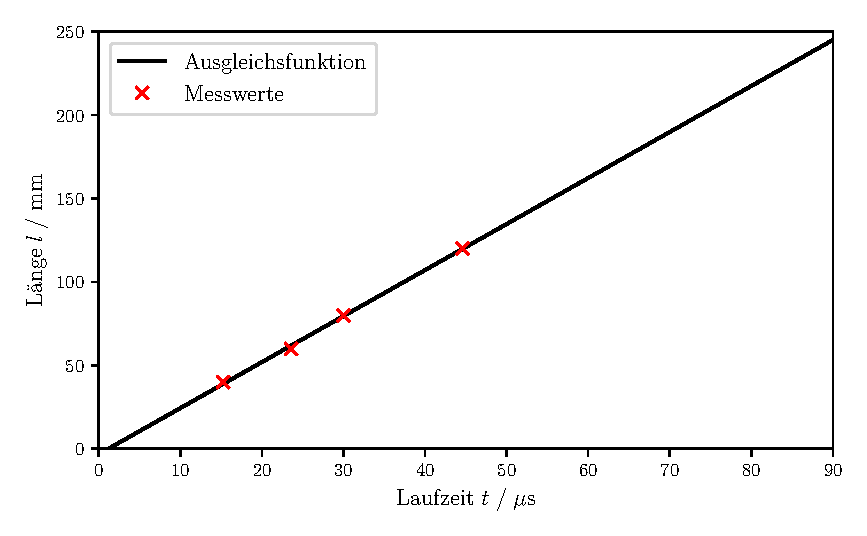
\includegraphics[width=15cm]{messwerte/Durchschallung.pdf}
    \caption{Zylinderhöhe $l$ geplottet gegen die Laufzeit $t$ beim Durchschallungs-Verfahren.}
    \label{fig:Durchschallung}
  \end{figure}
  Mit Python wird nun erneut Steigung und y-Achsenabschnitt bestimmt. Die Steigung entspricht erneut der 
  Schallgeschwindigkeit in Acryl $c_{\mathrm{Acryl}}$ und der y-Achsenabschnitt der Anpassungsschicht $d$.
  \begin{align*}
    c_{\mathrm{Acryl}} &= (2,75913 \pm 0,07181) \, \si{\milli\meter\per\micro\second} &= (2759,13 \pm 71,81) \, \si{\meter\per\second} \\
    d &= (-3,25 \pm 2,18) \, \si{\milli\meter} &= (-3,25 \pm 2,18) \cdot 10^{-3} \, \si{\meter}
  \end{align*}
  Die Messwerte und Ausgleichsfunktion sind in \autoref{fig:Durchschallung} dargestellt.

\subsection{Bestimmung der Dämpfung mit dem Impuls-Echo-Verfahren}

  Für die Bestimmung der Dämpfung der Ultraschallwellen in Acrylglas, werden die Messwerte 
  aus \autoref{tab:EchoImpuls} verwendet.\\
  Zwischen Dämpfung und Amplituden besteht der Zusammenhang aus \autoref{eqn:Dämpfung}. Diese Gleichung wird
  zu
  \begin{equation*}
    \log{\frac{U}{U_0}} = -\alpha \cdot 2 \cdot l
  \end{equation*}
  umgestellt, damit eine Ausgleichsrechnung mittels Python durchgeführt werden kann.\\
  Der letzte Messwert der Amplituden wird ignoriert, da dieser stark von den anderen abweicht und auf einen
  Messfehler hindeutet.\\
  Mittels Python wird die Steigung, die Dämpfung, bestimmt und anschließend in \autoref{fig:Daempfung} geplottet.
  Die Dämpfung beträgt somit $\alpha = (23,2 \pm 3,2) \, \si{\per\meter}$.

  \begin{figure}
    \centering
    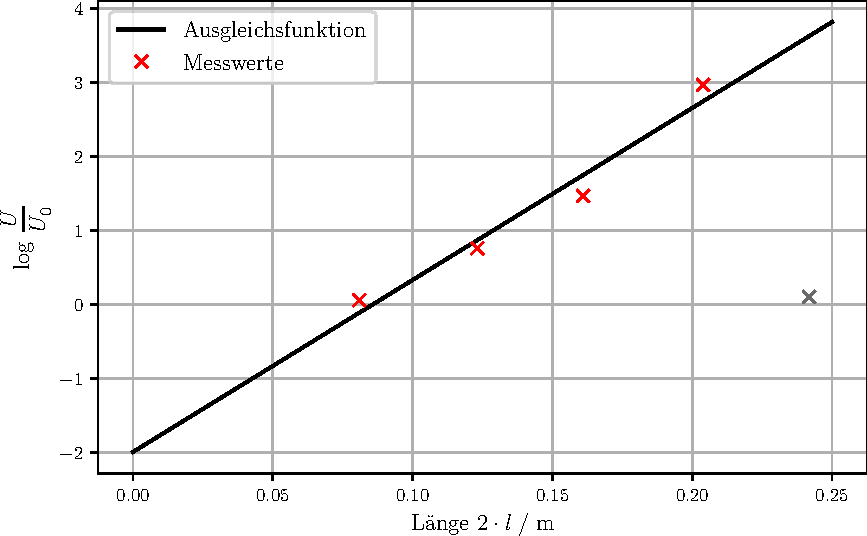
\includegraphics[width=15cm]{messwerte/Daempfung.pdf}
    \caption{Halblogarithmische Darstellung der Amplitudenverhältnisse gegen die zurückgelegte Strecke innerhalb der Acrylzylinder.}
    \label{fig:Daempfung}
  \end{figure}

\subsection{Biometrische Untersuchung eines Augenmodells}

  In dieser Versuchsreihe wird ein Augenmodell mittels Impuls-Echo-Verfahren durchschallt.\\ 
  Im Programm zur Visualisierung des Schalls lassen sich vier deutliche Haupt-Peaks erkennen.
  Diese sind der Iris, Ein- und Austreten der Linse und der Retina zuzuordnen.\\
  Bei der Auswertung muss darauf geachtet werden, dass in dem Glaskörper, der Augenkammer und der 
  Linse jeweils unterschiedliche Schallgeschwindigkeiten herrschen.\\
  Das Kammerwasser der Augenkammer kann mit Wasser angenähert werden $c_{\mathrm{Wasser}} = 1492 \, \si{\meter\per\second}$  \cite{medizinphysik}.
  Die Schallgeschwindigkeit in der Linse beträgt $c_{\mathrm{L}} = 2500 \, \si{\meter\per\second}$ und in der
  Glaskörperflüssigkeit $c_{\mathrm{GK}} = 1410 \, \si{\meter\per\second}$ \cite{sample}, wie bereits in der Durchführung erwähnt.\\
  Die Messwerte sind in \autoref{tab:Auge} aufgelistet.

  \begin{table}
    \centering
    \caption{Beim Untersuchen des Augenmodells aufgenommene Daten.}
    \label{tab:Auge}
    \begin{tabular}{c | c c}
      Peak & Laufzeit $t$ / $\si{\micro\second}$ & Amplitude $U$ / $\si{\volt}$ \\
        \midrule
        1   & 10,38 & 0,7614\\
        2   & 15,74 & 0,7179\\
        3   & 22,50 & 0,1633\\
        4   & 72,04 & 0,1088\\
        \bottomrule
      \end{tabular}
  \end{table}

  Mittels der \autoref{eqn:Strecke} und Python werden nachfolgende Distanzen bestimmt.

  \begin{align*}
    \mathrm{Hornhaut \,\, zu  \,\, Iris} &= 0,77 \, \si{\centi\meter}\\
    \mathrm{Iris \,\, zu \,\, Anfang \,\, Linse} &= 0,39 \, \si{\centi\meter}\\
    \mathrm{Dicke \,\, Linse} &= 1,65 \, \si{\centi\meter}\\
    \mathrm{Ende \,\, Linse \,\, bis \,\, Retina} &= 2,27 \, \si{\centi\meter}\\
  \end{align*}
